\documentclass{article}

\usepackage[utf8]{inputenc}

% Packages
\usepackage{amsmath,amssymb}
\usepackage{bm}% boldmath
\usepackage{listings} % Code block (source code) \begin{lstlisting} 
\usepackage{natbib}
\usepackage{graphicx}
\usepackage{lmodern}
\usepackage[usenames,dvipsnames,svgnames,table]{xcolor}
\usepackage[textwidth=16cm,textheight=23cm]{geometry}

%\usepackage{inconsolata} % New monospace font

% URL
\usepackage{url}
\usepackage[colorlinks=true, a4paper=true, pdfstartview=FitV, linkcolor=blue, citecolor=blue, urlcolor=blue]{hyperref}

% Figures
\usepackage[font=small, labelfont=bf]{caption}
\usepackage{subfig} % Subfigures. Uses \subfloat[captions text]{figure}

% Tables
\usepackage{booktabs}   % Allows the use of \toprule, \midrule and \bottomrule in tables for horizontal lines
\newcommand{\ra}[1]{\renewcommand{\arraystretch}{#1}} % spaces in tables

% Itemize
\usepackage{enumitem}

% Commands
%\newcommand{\code}[1]{\texttt{#1}} % \code{inline code}
\newcommand{\code}[1]{{\small\ttfamily #1}} % \code{inline code}
\newcommand{\expval}[1]{\langle #1 \rangle} %
\renewcommand{\theequation}{\arabic{section}.\arabic{equation}} % Book format equation
\renewcommand{\thefigure}{\arabic{section}.\arabic{figure}} % Book format figure
\renewcommand{\vec}[1]{{\bf #1}} % Lars likes this better than arrow

% Set page attribution
\setlength{\parindent}{0pt}


% PSTRICKS
\usepackage{pstricks,pst-node,pst-tree} % includes graph additions
\usepackage{pst-pdf} % Compiles the pictures
\usepackage{pst-node}
\usepackage{pst-plot}
\usepackage{pst-3dplot}
%\usepackage{pstricks-add,babel}




\lstset{
language=Python,                        % Code langugage
commentstyle=\color{gray},              % Comments font
basicstyle=\small\ttfamily,             % Code font, Examples: \footnotesize, \ttfamily
keywordstyle=\bfseries\color{blue},
stringstyle=\color{orange},
numbers=left,                           % Line nums position
numberstyle=\tiny,                      % Line-numbers fonts
stepnumber=1,                           % Step between two line-numbers
numbersep=5pt,                          % How far are line-numbers from code
frame=none,                             % A frame around the code
tabsize=4,                              % Default tab size
captionpos=b,                           % Caption-position = bottom
breaklines=true,                        % Automatic line breaking?
breakatwhitespace=false,                % Automatic breaks only at whitespace?
showspaces=false,                       % Dont make spaces visible
showstringspaces=false,                 % Dont make spaces visible in strings
showtabs=false,                         % Dont make tabls visible
belowskip=8pt,
morekeywords={range, xrange},
% backgroundcolor=\color{yellow}
% emph={[2]root,base}
% morekeywords={one,two,three,four,five,six,seven,eight,
}


%commentstyle=\color{gray},              % Comments font
%basicstyle=\small,                      % Code font, Examples: \footnotesize, \ttfamily



%basicstyle=\footnotesize\ttfamily,
%keywordstyle=\bfseries\color{green!40!black},
%commentstyle=\itshape\color{purple!40!black},
%identifierstyle=\color{blue},
%stringstyle=\color{orange},







% ***************************************************
% HEADER INFORMATION

\title{Exercise 2}
\author{Molecular Statistics, Week 2}
\date{2014}

% ***************************************************

\begin{document}


% ***************************************************
% BEGIN DOCUMENT
% ***************************************************

\maketitle

\section{Introduction}

This is the second exercise in the course Molecular Statistics.
%
The exercises
in this course are split in two parts. The first part of each exercise is a
general introduction to new concepts and programming techniques in the python
programming language, which covers and extends what is written in the
curriculum.
Just like last week.\\

The curriculum can be found here 
\href{http://pymbook.readthedocs.org/en/latest/}{pymbook.readthedocs.org/en/latest},

Read the following chapters for this week

\begin{itemize}
    \item \href{http://pymbook.readthedocs.org/en/latest/functions.html}{functions} 
          \newline to and including "Keyword arguments". Ignore the rest.
\end{itemize}


\section{Functions}

Last week, the computer program you wrote was executed line by line in a top to
bottom approach, i.e. the programs way of execution is easily followed by just
reading the source file as you would read a book. It turns out, however, that
when the programs become large enough, it is no longer a clever way to organize
your program since you'll eventually loose track of what is going on. What one
usually does is to break up the program into logical parts, such as “Initialize
particles”, “perturb the particles” and “calculate properties”. Today's
exercise is an exercise in restructuring the code
from last week into logical parts which we can easily distinguish. Before we
get to the exercise, however, we shall have a look at functions, which are
essential in this process.\\

As in mathematics, functions in any programming language can be seen as a
means to get a predefined output based on some input. Also, just as in
mathematics, functions can have several variables, but in programming languages
such as python, you can essentially parse anything into these
functions, i.e. lists, floats, text and even your own data types. We'll start with some simple functions that arise in mathematics and
continually extend upon them until you are ready to start with the exercise.\\

They function $f(x)=x^2$ is a good example of how you can turn mathematics into code in python without much hassle.

\begin{lstlisting}
def f(x):
    y = x * x
    return y
\end{lstlisting}


\begin{enumerate}
  \item Insert the above code into your text file, save and execute. What
      happens? Can you explain why? {\em Hint:} Nothing happens right now. Why?
\end{enumerate}

In programming languages you provide the {\em definition} of a function, and
just like on your calculator you need to {\em call} those functions before they
are actually executed.

\begin{enumerate}
  \setcounter{enumi}{1}
  \item Below the code you wrote above, insert the following lines of code and
    explain what happens when you run the script

\begin{lstlisting}
print f(-1.0)
print f(0.0)
print f(1.0)
print f(2.0)
\end{lstlisting}

  \item Instead of printing directly as you did in (2), assign the values of
    the functions to variables and print them afterwards, i.e. \code{a =
    f(6.0)}.

\end{enumerate}

The reality is that our custom functions actually works like the built in
functions in python (remember the \code{len(arg)} function from last week for instance)
,so once you know how to make one, you can essentially create as many you like.\\

To test functions we would need a list of $x$-values as input.
We could use the \code{range()} function from last week, but that would limit us to
integers. Instead we use a very useful tool call NumPy which is imported as all other tools;

\begin{lstlisting}
import numpy
\end{lstlisting}

We can then use the \code{arange(start, end, step)} function.
This will produce a list just like the \code{range()} function, but this time the
\code{start},
\code{end}, and
\code{step}
can be floats instead of only integers.

\begin{lstlisting}
x_list = numpy.arange(0, 10, 0.1)
\end{lstlisting}

\begin{enumerate}
  \setcounter{enumi}{3}
  \item Define the following function using \code{numpy.exp()}.
    \begin{align}
        h(x) = \frac{1}{x} + e^{5x}
    \end{align}

  \item Define a list of $x$-values, ranging from -1 to 1 with a step size of 0.1, using the \code{arange()} function.

  \item Plot the result using pylab.

\end{enumerate}

Next let us plot something more complex. Use \code{numpy.sin()} and \code{numpy.cos()}.

\begin{enumerate}
  \setcounter{enumi}{6}
  \item Define the following two functions
    \begin{align}
        q(t) = 13\sin(t)^3 && \text{and} && p(t) = 13\cos(t) - 5 \cos(2t) - 2 \cos(3t) - \cos(4t)
    \end{align}

  \item Define a list of $t$-values from $-2\pi$ to $2\pi$.
      {\em Hint:} Use \code{numpy.pi} to get the values of $\pi$.

  \item For each value of $t$, plot $p(t)$ vs. $q(t)$, with $p(t)$ as the $y$-value and $q(t)$ as the $x$-value.

\end{enumerate}

\newpage
\section{Interacting particles - The Hard Sphere Model}

Goal of today

\begin{itemize}
  \item Restructure the program from last week using functions.
  \item Allow the particles to interact by measuring the distance from all the other particles
    and if two particles are close make a reflection.
  \item Count particles and estimate when an equilibrium condition has been established.
\end{itemize}

As a starting point for your code, you should copy over your solution to last
weeks exercise. If you didn't finish the exercises last week, download the file
\code{week1\_solution.py} from Absalon. The following code should be seen as
inspiration for how the code should be structured after this exercise is done.

\begin{lstlisting}
import random
import pylab
import video # 2d Video

def distance(xi, yi, xj, yj):
    """ Calculate the distance between particle i and particle j
    """
    return d


def initialize_particles(n_particles):
    """ Initialze particles, positions and velocities
    """
    return pos_x, pos_y, vel_x, vel_y


def simulate_step(pos_x, pos_y, vel_x, vel_y, dt):
    """ Here we simulate a step dt for all particles.
    """
    return pos_x, pos_y, vel_x, vel_y


def plot_particles(X, Y, filename):
    """Insert code to save a picture
    of the particle positions
    """


# Run the simulation
n_particles = 40
n_steps = 10000
dt = 0.001
X, Y, Vx, Vy = initialize_particles(n_particles)

plot_particles(X, Y, 'coordinates_start.png')

for n in range(n_steps):
    X, Y, Vx, Vy = simulate_step(X, Y, Vx, Vy, dt)

    if n % 10 == 0:
        video.add_frame(X, Y)

plot_particles(X, Y, 'coordinates_end.png')
video.save('exercise_2')

\end{lstlisting}

\newpage
Important Note.
Notice how the bottom part of the script is the code that actually calls the
appropriate functions to make the simulation.  This makes reading the overall
structure of the program easier because you can now see how the program is
executed and then inspect the appropriate functions.  Also, it is not important
in what order your functions are defined. What matters is the order in which you
call them. This is.different than i.e. variables, which have to be defined and have a value assigned before you use them.

\begin{enumerate}
  \setcounter{enumi}{0}
  \item Inspect the above code and restructure your own code from last week to have the
    same structure and functions.
\end{enumerate}

Remember that this is only done because it is easier to read and in
the end, it is up to yourself to decide how you want to structure your
programs.

\begin{enumerate}
  \setcounter{enumi}{1}
  \item Finish the function \code{distance()} and make it return
    the distance \code{d} between particle $i$ and $j$.

  \item Extend your program to create a new variable $r_{min}$ and set its
    value to 0.03.
    This is the distance that the two particles $i$ and $j$ have to be within
    in order to make a reflection.

% TODO Reflection = elastic impact

\end{enumerate}

We need to get the interaction between all the possible particle pairs.
By looping over each particle twice, we can get all the possible interactions.

\begin{lstlisting}
for i in range(n_particles):
    for j in range(n_particles):
        print "Interacting particles", i, "and", j
\end{lstlisting}

Since the particles are interchangable, this will count each interaction twice.
We also want to skip the interaction if particle $i$ is the same as $j$.
All this can be solved by a simple \code{if}-statement.

\begin{lstlisting}
if i > j:
    print "Interacting particles", i, "and", j

\end{lstlisting}

\begin{enumerate}
  \setcounter{enumi}{3}
  \item Before implementing the solution, check that the above loop and
    if-statement works as expected, and checks all unique interactions only once. {\em Hint: Use
    a print statement.}

  \item Modify your code to loop over all particle interactions. Print the
    distance between the two particles interacting.

\end{enumerate}

% TODO move to earlier
To let the particles interact, we will use a simple model. The
particles are considered as being small disks with a diameter of $r_{min}$ and they have
perfect elastic scattering when particle $i$ comes into contact with particle $j$.
(Think a game of billiards)

% Deleted stuff about assuming the particles being very small, since it seemed confusing.

When two particles collide elastically they will exchange velocities which is done by simply setting

\begin{align}
  \vec{v}_i = \vec{v}_j & & \text{and} & & \vec{v}_j = \vec{v}_i
\end{align}

%TODO The x/y-components of the velocity should change relative to the vector from particle i's center to particle j's.
% I'm assuming that this comes later, but there should be a note about that we assume that all collisions are head-on.
% I'm just too tired to figure it out atm, so must do later.

\begin{enumerate}
  \setcounter{enumi}{5}
  \item Implement in your code this exchange of velocities for particles upon
    collision. Use the following if-statement as inspiration.
    {Hint:} Save the velocity of particle $i$ in a temporary variable.

\begin{lstlisting}
if d < r_min:
    # Collision
\end{lstlisting}

\end{enumerate}

As a final part of todays exercise, we can extract some useful information from the simulation.
Since the system we are investigating is not the most physical correct one and
particle positions do tend to be a bit boring by themselves, we shall instead
sample a property, which shows that the system is indeed random.

\begin{enumerate}
  \setcounter{enumi}{6}
  \item For each 5 steps in your simulation, calculate the number of particles
    that are present in the interval $x \in [0, 1]$.
    Append that number to a list named \code{partdist}.  To get proper results,
    you need to change \code{n\_steps} to 20000 and \code{n\_particles} to 40.

    {\em Note:} Remember to disable saving of the video when running with large
    steps!

\end{enumerate}

We want a histogram of how often $N$ particles occurred in the above
interval. So along the $x$-axis should give you the number of particles we have
encountered in the interval, and along the $y$-axis how oftern that number
has occurred.\\

To plot the information from the list we can use the pylab histogram as follows

\begin{lstlisting}
pylab.hist(partdist, bins=range(0, n_particles), align='left')
pylab.savefig('dist_histogram.png')
\end{lstlisting}

which is inserted after the main loop over \code{n\_steps}.

\begin{enumerate}
  \setcounter{enumi}{7}
  \item Plot the histogram and comment on the results, i.e. how is the
    distribution of particles in interval?

  \item Make another list named \code{partdisteq}. Here you should store the
    number of particles in the same interval as above, but only {\bf after}
    10000 calibration steps have passed. Plot it on a new figure and comment
    on the result.

\end{enumerate}

\begin{figure}[htb]
  \subfloat[Before equilibrium steps]{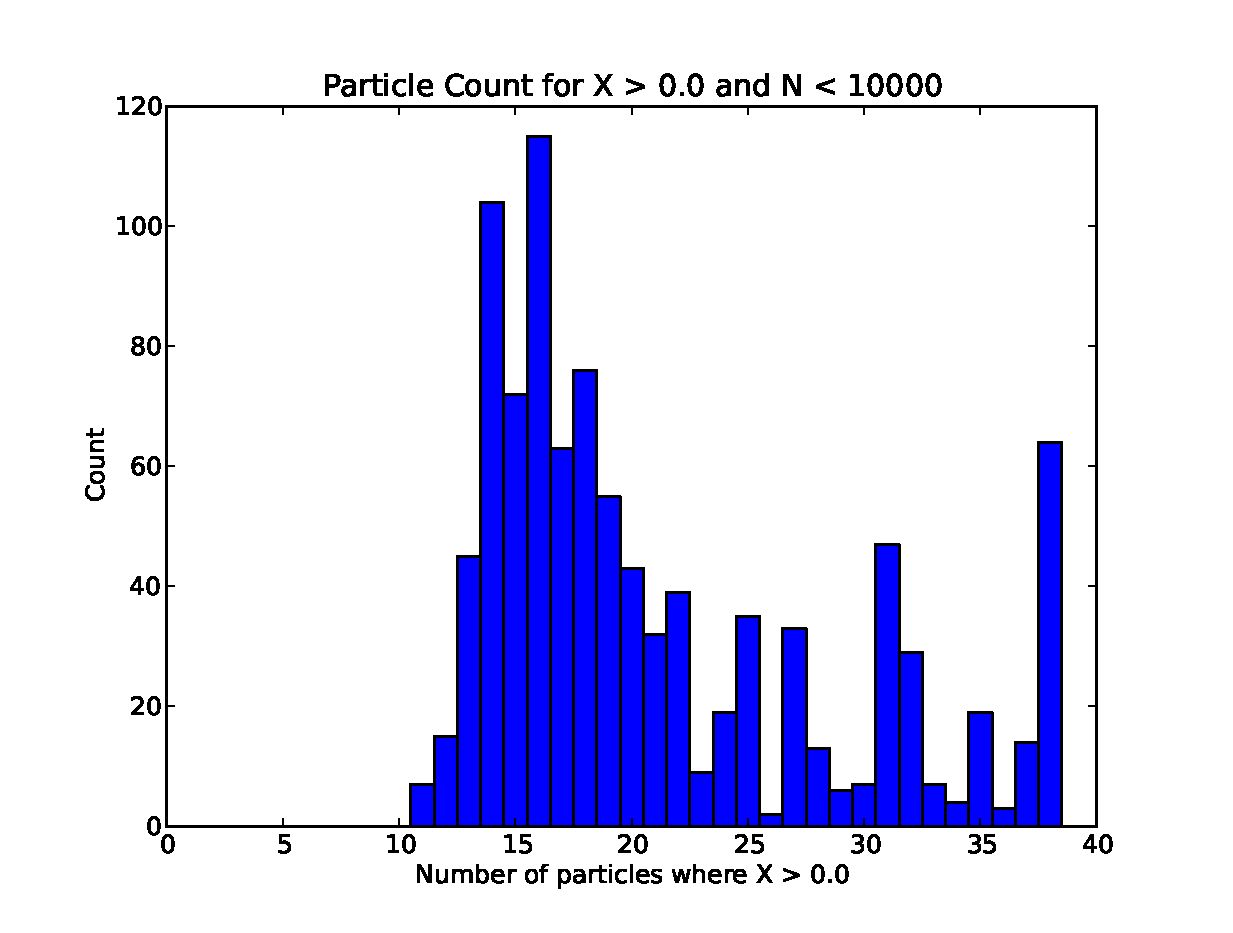
\includegraphics[width=0.5\textwidth]{partdist.eps}}
  \subfloat[After equilibrium steps]{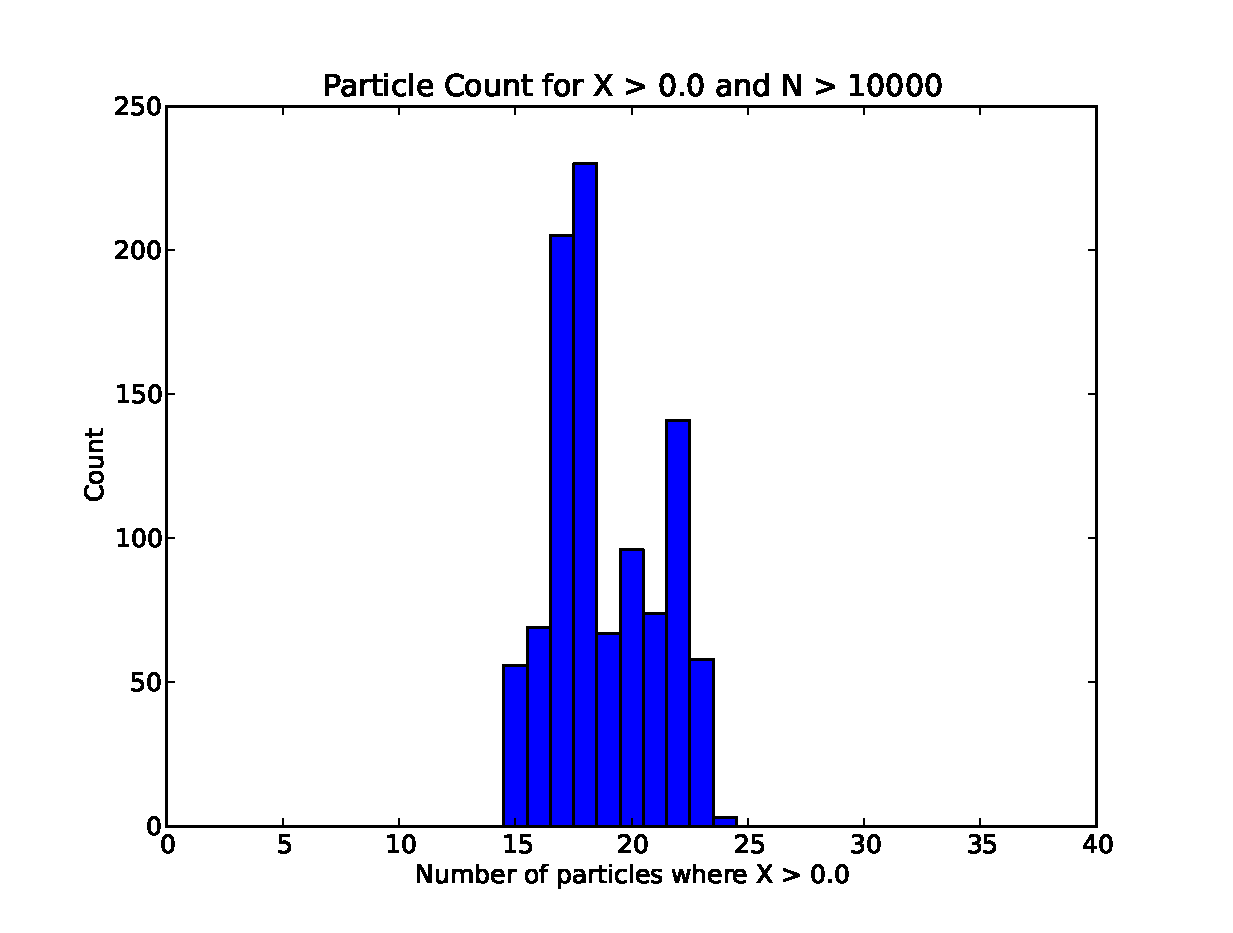
\includegraphics[width=0.5\textwidth]{partdisteq.eps}}
  \label{fig:partdist}
  \caption{
     Count of the number of particles placed to the right in a container in the
     before and after equilibrium steps.
  }
\end{figure}



% ***************************************************
% END DOCUMENT
% ***************************************************

\end{document}

